\documentclass[10pt,a4paper]{article}
\usepackage[utf8]{inputenc}
\usepackage[T1]{fontenc}
\usepackage[spanish]{babel}
\usepackage{amsmath}
\usepackage{amsfonts}
\usepackage{amssymb}
\usepackage{graphicx}
\usepackage{float}
\usepackage{multicol}
\usepackage[dvipsnames]{xcolor}
\usepackage{hyperref}
\definecolor{pinegreen}{rgb}{0.36, 0.54, 0.66}
\hypersetup{
    colorlinks=true,
    linkcolor=pinegreen,      
    urlcolor=red,
    }
\addto{\captionsspanish}{\renewcommand{\abstractname}{Abstract}}
\newcommand{\celda}[1]{
	\begin{minipage}{2cm}
		\vspace{2mm}
		#1
		\vspace{2mm}
	\end{minipage}
}
\definecolor{pinegreen}{rgb}{0.36, 0.54, 0.66}
\usepackage[left=2.00cm, right=2.00cm, top=2.00cm, bottom=2.00cm]{geometry}
%-----------------------
\usepackage{fancyhdr}
\usepackage{lastpage}   
\pagestyle{fancy} 
\fancyhf{}   
\rhead{Gabriel Hernández}                       %Create right header text
\chead{Medición de la capacidad de un DVD}  
\lhead{Laboratorio 2}                        %Create left header text
                   %Create center header text

\rfoot{Page \thepage \hspace{1pt} of \pageref{LastPage}}    %Create right footer text
\renewcommand{\headrulewidth}{0.2pt}      %Set header line thickness to 0 pt [default=1pt]
\renewcommand{\footrulewidth}{0pt}      %Set footer line thickness to 0 pt [default =0pt]
%-----------------------
\author{Gabriel Hernandez Bello}
\begin{document}
	
	\begin{figure}[H]
		\raggedright
		
\includegraphics[scale=0.2]{../Altura-Campanil/IMG/logo_udec.png} \hfill 
\includegraphics[scale=0.5]{../Altura-Campanil/IMG/cfm_logo.png}
	\end{figure}

	\vspace{6mm}
	%ESTE CENTER ES EXCLUSIVO PARA EL TITULO DEL PAPER, AUTOR Y UNIVER.
	\begin{center}
		{\Large \textbf{Medición de la capacidad de un DVD}}\\
		\vspace{2mm}
		{\large Gabriel Hernández Bello$^{1}$}\\
		\vspace{6.5mm}
		$^1$\textit{Universidad de Concepción, Facultad de Ciencias Físicas y Matemáticas, Ciencias Físicas. }\\
	\end{center}

	\begin{center}
		\textcolor{pinegreen}{\rule{150mm}{0.8mm}}
	\end{center}

      %ESTE ABSTRACT ES PARA EL RESUMEN PROPIAMENTE DICHO Y PARA LAS PALABRAS CLAVES (KEYWORDS) ,NOTA:el comando \par sirve para iniciar el nuevo parrafo con sangría.
	\begin{abstract}
	A partir de conceptos fundamentales en física óptica diseñamos un montaje experimental para determinar la capacidad de un DVD-R de 4.7 [GB] de almacenamiento. El experimento se basó en la estimación del espaciado entre los surcos que conforman el disco óptico para luego calcular la capacidad.\\
	Las estimación obtenidas indicaron una  capacidad de 4.43 $\pm$ 0.07 [GB] para un láser  con longitud de onda $\lambda_r = 650$[nm]  (rojo) y  4.82 $\pm$ 0.07 [GB]  para un láser con longitud de onda $\lambda_v = 530$[nm] (verde). Estos valores presentaron un error relativo del 5.7 $\%$  para el láser rojo y 2.6 $\%$ para el láser verde, validando el proceso experimental y el tratameinto de los datos.\\
	\\
		\textbf{Palabras Claves ---}  DVD, Láser, Patrón de Difracción, Óptica.
	\end{abstract}
	
	\begin{center}
		\textcolor{pinegreen}{\rule{150mm}{0.8mm}}
	\end{center}
	
	\begin{multicols}{2}
		\section{Introducción}
			El DVD es un disco óptico para almacenamiento de datos. Las siglas DVD corresponden a \emph{Disco Versátil Digital}. Fue creado y desarrolloado en 1995 con su primer lanzamiento para 1 Noviembre de 1996, en Japón. El medio puede almacenar cualquier tipo de datos digitales y se ha utilizado ampliamente para almacenar programas de vídeo (vistos con reproductores de DVD), software y otros archivos informáticos. Los DVD ofrecen una capacidad de almacenamiento significativamente mayor que los discos compactos (CD) aunque tienen las mismas dimensiones. Un DVD estándar de una sola capa puede almacenar hasta 4,7 GB de datos, un DVD de doble capa hasta 8,5 GB. Las variantes pueden almacenar hasta un máximo de 17,08 GB \cite{wikiDVD}.\\
			
			En este laboratorio trabajaremos con un DVD de capa simple y aprovecharemos sus caracterísitcas ópticas para estimar su capacidad.
		\section{Marco Teórico}
		\subsection*{Especificaciones del DVD}
		Los DVD almacenan información en una línea de \emph{surcos} microescópicos dispuestos en una espiral que va desde el centro del disco hacia la circunsferencia exterior. Así, todos los lectores de DVD utilizan láseres para leer la información codificada en los surcos. La longitud de onda del láser depende de la separación de los surcos, en general esta es de 0.74 [$\mu m$].\\
		
		Los DVD constan de tres capas: el sustrato de policarbonato transparente, la capa de colorante y la capa reflectante. En partícular, la capa de reflexión se encuentra en medio de las capas de policarbonato. La más importante es la capa de reflexión que consta, en la mayoría de los casos, de una lámina de aluminio que vuelve la superficie del DVD relfectante. Lo anterior permite que el láser del lector se refleje para ser leído por el sensor de recogida de la unidad fotocaptora. \cite{especificaciones_DVD}.
		\subsection*{Interferencia} 
		Se habla de interferencia cuando dos o más ondas coinciden en la misma región del espacio en el mismo instante de tiempo. Luego, la función de onda total es la suma de las funciones individuales (Principio de SUperposición), no así la intensidad de total de la onda. En el caso particular de dos ondas, la intensidad de la onda resultante queda expresada por la \emph{ecuación de interferencia}:
		\begin{equation}
		I = I_1 + I_2 + 2\sqrt{I_1 I_2} \cos(\varphi),
		\end{equation}
		donde $\varphi = \varphi_2 - \varphi_1$ representa el factor de \emph{desfase} entre las ondas \cite{interferencia}.
		\subsection*{Difracción}
		En términos simples, la difracción es la curvatura de una onda alrededor de los bordes de una abertura o un obstáculo. Este fenómeno lo presentan todos los tipos de ondas. En particular, cuando la onda pasa por una rejilla se forma un \emph{patrón de difracción} caracterizado por máximos (puntos luminosos) y mínimos (puntos oscuros) de intensidad. Asimismo, es posible definir analíticamente los puntos de interfencia destructiva (minimos) ocasionados por una rejilla, a través de la siguiente expresión:
		\begin{equation}\label{minimos de intensidad}
		d \sin(\theta_n) = n \lambda, \hspace{5mm} n = \pm 1, \pm 2, \pm 3,... 
		\end{equation}
		Donde $d$ es el ancho de las ranuras en la rejilla, $\theta_n$ es el ángulo de incidencia que produce la intensidad mínima y $\lambda$ es la longitud de la onda \cite{wikidifrac}.
		\subsection*{Trigonometría}
		Etimológicamente la palabra trigonometría significa \textit{medida de los triángulos}. En efecto, es la ciencia que estudia las relaciones que ligan los lados de un triángulo y aplican esas realciones al cálculo de los elementos desconocidos. En particular, la trigonometría se basa en el conocimiento de los ángulos de un triángulo que establecen conexiones llamadas \textit{relaciones trigonométricas}. Las principales son el \emph{seno, coseno} y la \emph{tangente} \cite{trigonometria}.
		\section{Procedimiento Experimental y Resultados}
		Para este experimento utilizamos un DVD de una capa, compuesto por una capa vacía y otra con información (en adelante \emph{capa/disco óptico}). Luego separamos ambas capas del DVD para trabajar únicamente con el disco que contiene toda la infomación, es decir, los surcos. Después, colocamos una pantalla de observación atrás del disco óptico y apuntamos un láser hacia este generando un patrón de difracción, visible en la pantalla, a causa de los surcos que componen la capa óptica. Para asegurar la estabilización del láser utilizamos un soporte universal.\\
		
		Experimentalmente medimos la distancia entre el DVD y la pantalla de observación ($d$), así como el espaciado de los surcos observado en el patrón de difracción ($L$), en particular, medimos la separación entre el has de luz original (orden $n=0$) y el primer mínimo de interferencia visible en la pantalla (orden $n=1$). Finalmente, calculamos el ángulo de apertura ($\theta$) para la posterior estimación de la separación entre los surcos en el disco óptico ($D$), (Figuras \ref{imagen laser verde} y \ref{imagen laser rojo} ). \\
		El valor del ángulo $\theta$ fue calculado mediante la siguiente expresión:
		\begin{equation}
		\tan(\theta) = \frac{L}{d} \Longrightarrow \theta = \arctan(\frac{L}{d}).
		\end{equation}
		Esta relación se puede apreciar mejor en la figura \ref{Diagarama} donde se explicita la relación entre las distancias y el ángulo en cuestión.\\
		A continuación, utilizamos el concepto de patrón de difracción para estimar la separación entre los surcos. Para ello, notemos que $L$ representa la distancia hasta el primer mínimo de interferecia. Esto ímplica que trabajamos para n=1 en la expresión \ref{minimos de intensidad}, es decir:
		\begin{equation}
		D = \frac{\lambda}{\sin(\theta)}, \hspace{2mm} n = 1.
		\end{equation}
		\begin{figure}[H]
			\centering
			\includegraphics[scale=0.2]{Difracción.jpeg}
			\caption{Diagrama de la situación física del experimento. La red de difracción es generada por el DVD.}
			\label{Diagarama}
			\rule{80mm}{0.1mm}
		\end{figure}
	
		En los cuadros \ref{tab:angulos_distancias.} y \ref{tab:angulos_distancias 2.} se recogen los valores obtenidos para el exprimento realizado con un lasér de longitud de onda $\lambda_r = 650$[nm]  (rojo) y $\lambda_v = 530$[nm] (verde), respectivamente. Sin embargo, un laser rojo emite luz con una longitud de onda entre 620-750[nm], mientras que un láser verde oscila alrededor de 495-570 [nm] \cite{colors}. Luego, consideraremos un error asociado a la longitud de onda de 65[nm] para el láser rojo y 37.5 [nm] para el láser verde, es decir, la mitad de la diferencia de los extremos en el rango de valores asociado.\\
		
		Por otra parte, el error asociado a la medida del ángulo $\theta$ y el espaciado del surco $D$ son calculados de manera analítica con la siguiente fórmula \cite{error}:
		\begin{equation}\label{errores}
		\sigma^2 = \sigma^2_x \left( \frac{\partial f}{\partial x} \right)^2 + \sigma^2_y \left( \frac{\partial f}{\partial y} \right)^2 + \sigma^2_z \left( \frac{\partial f}{\partial z} \right)^2+...
		\end{equation}
		\newpage
		
		\begin{figure}[H]
			\centering
			\includegraphics[scale=0.1]{láser_verde.jpeg}
			\caption{Montaje experimental para el láser verde}
			\label{imagen laser verde}
			\rule{80mm}{0.1mm}
		\end{figure}
		
		\begin{figure}[H]
			\centering
			\includegraphics[scale=0.1]{láser_rojo.jpeg}
			\caption{Montaje experimental para el láser rojo}
			\label{imagen laser rojo}
			\rule{80mm}{0.1mm}
		\end{figure}
	
	
	
		
		
	\end{multicols}
	
	\begin{table}[H]
		\centering
		\begin{tabular}{|c|c|c|c|}
			\hline
			$d$ (m) & $L$ (m) & $\theta$ (rad) )&  $D$(nm) \\ \hline
			0.0240 $\pm$ 0.0005  & 0.034 $\pm$ 0.0005 &  0.95600 $\pm$ 0.00003  & 783.41 $\pm$ 0.44 \\
			0.0300 $\pm$ 0.0005  & 0.0440 $\pm$ 0.0005 &  0.97000 $\pm$ 0.00002 & 757.86 $\pm$ 0.44\\
			0.0400 $\pm$ 0.0005  & 0.0610 $\pm$ 0.0005 &  0.99000 $\pm$ 0.00002 & 765.52 $\pm$ 0.43 \\ 
			0.0500 $\pm$ 0.0005 & 0.0730 $\pm$ 0.0005 & 0.97000 $\pm$ 0.00001 & 775.86 $\pm$ 0.44\\ 
			0.0600 $\pm$ 0.0005 & 0.0890 $\pm$ 0.0005 & 0.97700 $\pm$ 0.00001 &  772.17 $\pm$ 0.44\\ 
			0.0700 $\pm$ 0.0005 & 0.1030 $\pm$ 0.0005 & 0.97300 $\pm$ 0.00001 & 774.27 $\pm$ 0.44\\
			0.0800 $\pm$ 0.0005  & 0.1190 $\pm$ 0.0005 &  0.97800 $\pm$ 0.00094 & 771.65 $\pm$ 0.44 \\ 
			0.0900 $\pm$ 0.0005 & 0.1360 $\pm$ 0.0005 &  0.98600 $\pm$ 0.00086 & 767.54 $\pm$ 0.44 \\
			0.1000 $\pm$ 0.0005 & 0.1550 $\pm$ 0.0005 &  0.99700 $\pm$ 0.00080 & 762.04 $\pm$ 0.44  \\
			0.1100 $\pm$ 0.0005 & 0.1640 $\pm$ 0.0005 &  0.97900 $\pm$ 0.00069 & 771.14 $\pm$ 0.44 \\
			0.1200 $\pm$ 0.0005 & 0.1720 $\pm$ 0.0005 &  0.96100 $\pm$ 0.00059 & 780.71 $\pm$ 0.45 \\
			0.1300 $\pm$ 0.0005 & 0.1860 $\pm$ 0.0005 &  0.96000 $\pm$ 0.00054 & 781.25 $\pm$ 0.45 \\
			0.1400 $\pm$ 0.0005 & 0.2030 $\pm$ 0.0005 &  0.96700 $\pm$ 0.00051 & 777,46 $\pm$ 0.45  \\
			0.1500 $\pm$ 0.0005 & 0.2200 $\pm$ 0.0005 &  0.97200 $\pm$ 0.00049 & 774.80 $\pm$ 0.45  \\ \hline
			
		\end{tabular}
		\caption{Ángulos y Distancias Medidas para el láser rojo}
		\label{tab:angulos_distancias.}
		\rule{100mm}{0.1mm}
	\end{table}
	
	\begin{table}[H]
		\centering
		\begin{tabular}{|c|c|c|c|}
			\hline
			$d$ (m) & $L$ (m) & $\theta$ (rad) )&  $D$(nm) \\ \hline
			0.0220 $\pm$ 0.0005  & 0.0240 $\pm$ 0.0005 &  0.82500 $\pm$ 0.00094 & 718.98 $\pm$ 0.44 \\
			0.0300 $\pm$ 0.0005  & 0.0320 $\pm$ 0.0005 &  0.81700 $\pm$ 0.00051 & 726.48 $\pm$ 0.44 \\
			0.0400 $\pm$ 0.0005  & 0.0420 $\pm$ 0.0005 &  0.80900 $\pm$ 0.00029 & 731.90 $\pm$ 0.43 \\ 
			0.0500 $\pm$ 0.0005 & 0.0550 $\pm$ 0.0005 & 0.83000 $\pm$ 0.00060 & 716.27 $\pm$ 0.44 \\ 
			0.0600 $\pm$ 0.0005 & 0.0660 $\pm$ 0.0005 & 0.83200 $\pm$ 0.00037 &  716.27  $\pm$ 0.44 \\ 
			0.0700 $\pm$ 0.0005 & 0.0770 $\pm$ 0.0005 & 0.83200 $\pm$ 0.00032 & 716.27 $\pm$ 0.44  \\
			0.0800 $\pm$ 0.0005  & 0.0850 $\pm$ 0.0005 &  0.81500 $\pm$ 0.00018 & 727.82 $\pm$ 0.44  \\ 
			0.0900 $\pm$ 0.0005 & 0.0980 $\pm$ 0.0005 &  0.82700 $\pm$ 0.00022 & 719.59 $\pm$ 0.44  \\
			0.1000 $\pm$ 0.0005 & 0.1090 $\pm$ 0.0005 &  0.82800 $\pm$ 0.00020 & 719.25 $\pm$ 0.44   \\
			0.1100 $\pm$ 0.0005 & 0.1200 $\pm$ 0.0005 &  0.82800 $\pm$ 0.00018 & 718.98 $\pm$ 0.44  \\
			0.1200 $\pm$ 0.0005 & 0.1310 $\pm$ 0.0005 &  0.82900 $\pm$ 0.00017 & 718.75 $\pm$ 0.45   \\
			0.1300 $\pm$ 0.0005 & 0.1430 $\pm$ 0.0005 &  0.83200 $\pm$ 0.00017 & 716.27 $\pm$ 0.45  \\
			0.1400 $\pm$ 0.0005 & 0.1510 $\pm$ 0.0005 &  0.82300 $\pm$ 0.00012 & 722.74 $\pm$ 0.45   \\
			0.1500 $\pm$ 0.0005 & 0.1610 $\pm$ 0.0005 &  0.82000 $\pm$ 0.00011 & 724.38 $\pm$ 0.45   \\ \hline
			
		\end{tabular}
		\caption{Ángulos y Distancias Medidas para el láser verde}
		\label{tab:angulos_distancias 2.}
		\rule{100mm}{0.1mm}
	\end{table}
\newpage
	\begin{multicols}{2}
	\section{Análisis}
	En las figuras \ref{Grafico laser rojo} y \ref{Grafico laser verde} se grafican los datos obtenidos para la separación de los surcos ($D$) y el ángulo de seperación desde el centro hasta el primer mínimo de intensidad  medidos para un láser rojo y uno verde, respectivamente. Además, se grafica la aproximación lineal de los datos para caso representado por la línea punteada. De ambas figuras podemos concluir que las variables gurdan una relación \emph{inversamente proporcional}. Esta correspondencia la podemos verificar en la ecuación \ref{minimos de intensidad}. Puesto que $n$ y $\lambda$ son constantes, a efectos del laboratorio, es de esperar que las variables $D$ y $\theta$ guarden una relación inversamente proporcional.\\
	
	 Notemos que la variación del espaciamiento del surco medido experimentalmente se ve restringida en el intervalo 773-795 [nm] para el láser rojo y 716-795[nm] para el láser verde. Por lo tanto, teniendo en cuenta que los valores se encuentran en un intervalo reducido, y por simplicidad; se considerará el valor promedio de los datos obtenidos en cada caso para estimar la capcidad del DVD. Estos son $D_r =785.5 \pm 5.9$ [nm] para el láser rojo y $D_v = 721.0 \pm  4.7$[nm] para el láser verde.\\
	 
	 Ahora bien, podemos estimar la capacidad del DVD considerando que el radio grabable del disco, medido experimentalmente, es de 3.7 $\pm$ 0.5 [mm]. Además, el \emph{valor real} del espaciamiento del surco aparece representado en la literatura con un valor de 740 [nm] \cite{wikiCD}. De lo anterior, podemos definir la \emph{denisdad lineal de surcos} como la cantidad de surcos por unidad de longitud (radio grabable del disco), tal que:
	 \begin{equation}\label{densidad}
	 \sigma = \frac{3.7\cdot 10^{-2} [m]}{740 \cdot 10^{-9} [m]} = 50000 
	 \end{equation}
	 
	 La relación \ref{densidad} representa que hay 50000 surcos por cada metro grabable en el DVD. En este sentido, dado que la capacidad real del disco es de 4.7 [GB], podemos relacionar los valores obtenidos experimentalmente con la capacidad estándar de 4.7 [GB] por cada 50000 surcos. De esta forma, obtenemos las densidades lineales de 47099.3 $\pm$ 478.2 para el láser rojo y 51317.6 $\pm$ 769.9 para el verde, lo que se traduce en capacidades de 4.43 $\pm$ 0.07[GB] y 4.82 $\pm$ 0.07[GB], respectivamente. Cabe mencionar que los errores de propagación, tanto de las densidades como de la capacidad resultante, fueron calculados con la expresión \ref{errores}. \\
	Por otra parte, sabemos que el valor real de almacenamiento del DVD es de 4.7 [GB], por lo tanto, podemos calcular el error asociado a los valores obtenidos para el láser rojo y verde. Así, obtenemos un error de 5.7 $\%$ para el láser rojo y de 2.6 $\%$ para el láser verde.
	
	\begin{figure}[H]
		\centering
		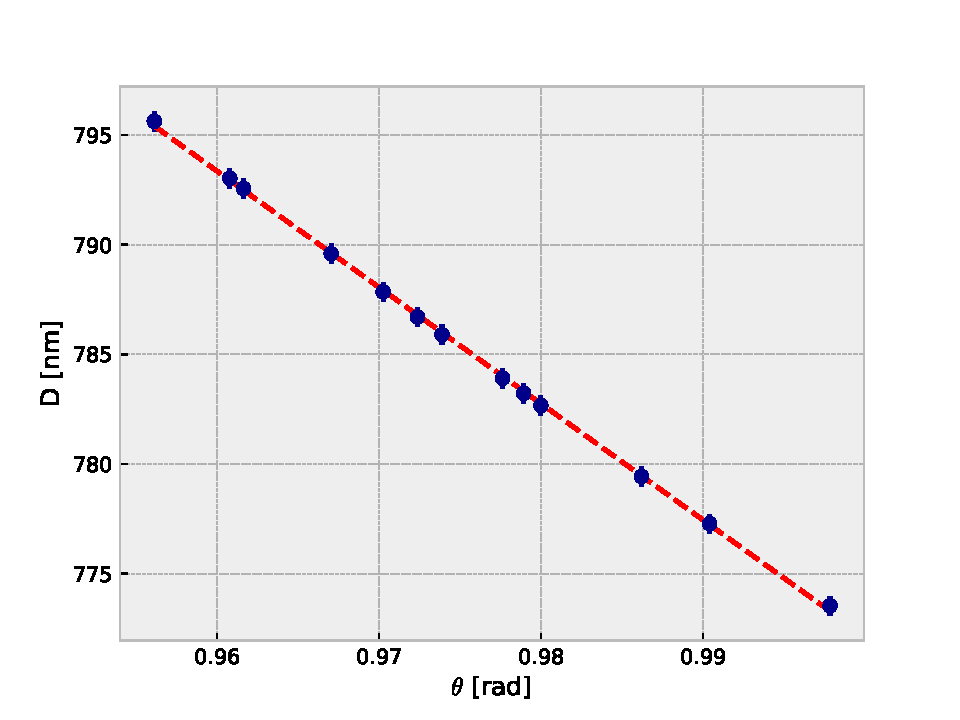
\includegraphics[scale=0.4]{laser_rojo.pdf}
		\caption{Gráfico del tamaño de los surcos del disco óptico en función del ángulo de desviación del láser rojo $\lambda_r = 650$[nm].}
		\label{Grafico laser rojo}
		\rule{80mm}{0.1mm}
	\end{figure}
	
	\begin{figure}[H]
		\centering
		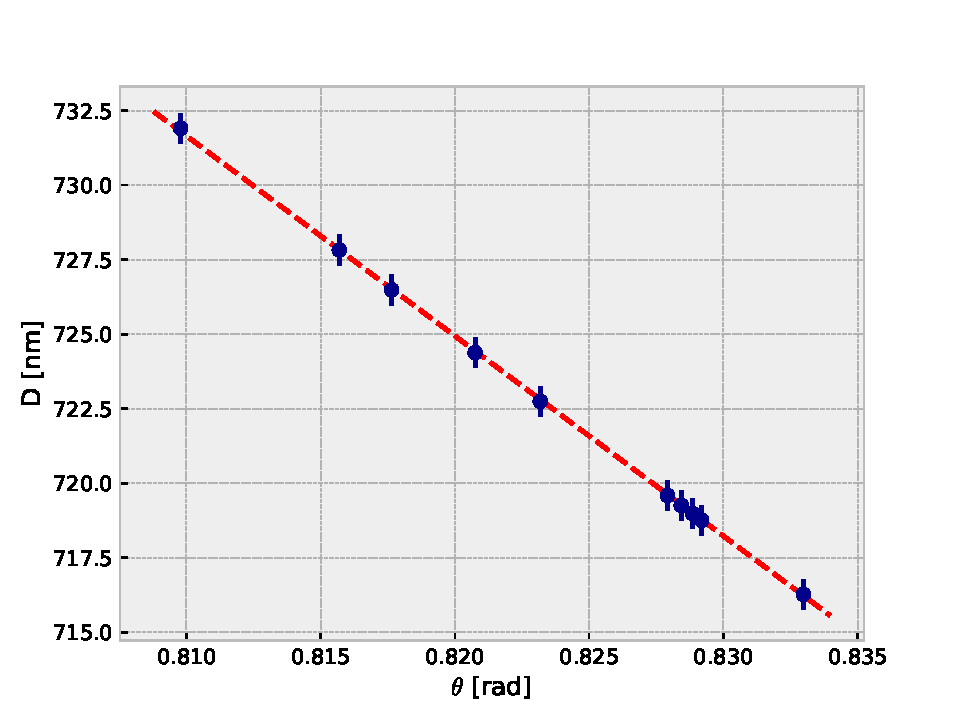
\includegraphics[scale=0.4]{laser_verde.pdf}
		\caption{Gráfico del tamaño de los surcos del disco óptico en función del ángulo de desviación del láser verde $\lambda_v = 530$[nm]. }
		\label{Grafico laser verde}
		\rule{80mm}{0.1mm}
	\end{figure}
	

	
\section{Conlusión}
En este laboratorio logramos estimar la capacidad de un DVD utilizando sus características ópticas a nuestro favor. Obtuvimos como resultado una capacidad de  4.43 $\pm$ 0.07[GB] para el láser rojo y 4.82 $\pm$ 0.07[GB] para el láser verde. Los valores estimados presentaron un error poco significativo de tan solo 5.7 $\%$  y 2.7 $\%$ para el láser rojo y  verde, respectivamente.  Argumentamos que los errores asociados a la medición son consecuencia de impresiciones en el proceso experimental, como la dispersión del láser o la falta de exactitud al  alejar el DVD de la pantalla.  No obstante, la baja magnitud de estos errores sugieren una correcta ejecución del experimento y un adecuado tratamiento de los datos. Rescatamos que el análisis presentado en el informe fue satisfactorio, aplicando conceptos fundamentales en óptica y ondas para determinar la capacidad del DVD, y obteniendo estimaciones cercanas al valor real. Además, los procedimientos seguidos fueron validados de forma coherente lo que reafirma la validez del enfoque experimental y los métodos utilizados para alcanzar el resultado final. 




	\bibliographystyle{unsrt}
	\bibliography{referencias}
	
	\end{multicols}
\end{document}